\begin{flushright} {\tiny {\color{gray} python\_codes/fieldstone\_130/text.tex}} \end{flushright}

%\lstinputlisting[language=bash,basicstyle=\small]{python_codes/fieldstone_130/keywords}

\begin{center}
\fbox{\textbf{\huge \color{teal} P}}
Codes at \url{https://github.com/cedrict/fieldstone/tree/master/python_codes/fieldstone_130}
\end{center}

\par\noindent\rule{\textwidth}{0.4pt}

%%%%%%%%%%%%%%%%%%%%%%%%%%%%%%%%%%%%%%%%%%%%%%%%%%%%%%%%%%%%%%%%%%%%%%%%%%%%%%%%%%%%%%%%%%%%%%

This is based on Simpson's book \cite{simp17}, chapter 7.3.

As an introduction to the topic of how the FEM can be
performed on systems of equations, we consider the following equations
\begin{eqnarray}
\frac{\partial A}{\partial t} &=& \Delta A  + \gamma (a-A+A^2B) \\
\frac{\partial B}{\partial t} &=& d \Delta B  + \gamma (b-A^2B) 
\end{eqnarray}
with the two unknowns, $A$ and $B$. This system of equations is used to model the interaction between
two interacting chemicals $A$ and $B$ \cite{mawb12}.

$B$ represents the concentration of
a ``substrate'' (inhibitor) chemical that is consumed in a reaction by some chemical ``activator'',
with concentration $A$. The reaction produces the activator, which explains the $A^2B$ terms in both
equations. Both substances are also produced at some background rate ($\gamma a$ for $A$ and $\gamma b$ for $B$,
respectively) and $A$ decays with first-order kinetics at a rate $\gamma$.

This ``substrate depletion'' reaction
model is known as Schnakenberg kinetics \cite{gime72,schn79}. This
model is most widely applied in biology, but it might also be relevant in Earth science to explain
the formation of self-organizing patterns, for example, related to mineral growth, stromatolites and
corals, concretions, and so on.

\begin{center}
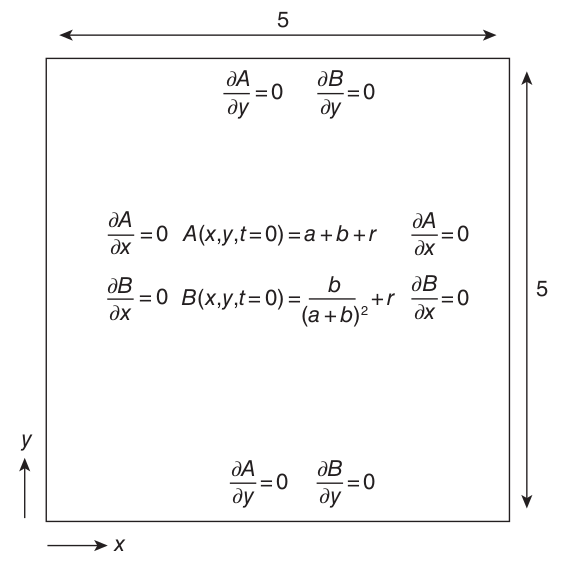
\includegraphics[width=5cm]{python_codes/fieldstone_130/images/simpson1}
\end{center}

The domain is a square of size 5. At $t=0$ the fields are given by
\begin{eqnarray}
A(x,y)&=&a+b+r \nn\\
B(x,y)&=& \frac{b}{(a+b)^2} +r
\end{eqnarray}
which is the steady-state solution with a small random perturbation $r$ (that has a maximum amplitude
of 1/100). No flux (zero gradient) conditions are considered across all lateral boundaries.

In the book we find: 
\begin{verbatim}
lx = 5 ; % length of x domain
ly = 5 ; % length of y domain
d = 20 ; % diffusivity of species B
a = 0.05 ; % growth rate of species A
b = 1 ; % growth rate of species B
gamma = 600 ; % kinetics
amp = 0.01 ; % max. amplitude of random noise
ntime = 200 ; % total number of time steps to compute
nxe = 50 ; % number of elements in x-direction
nye = 50 ; % number of elements in y-direction
dt = 5e-4 ; % time step
\end{verbatim}

The coupled PDEs are nonlinear: they both contain the term $A^2B$. As such 
a specific algorithm must be employed so as to make sure that the 
equations are adequately solved. Picard iterations are then used.
Since the matrix does not change (only the rhs) we will be making use of this fact.

\begin{eqnarray}
\int \vec{\bN}^T \vec{\bN} dV \cdot \frac{\partial \vec{\cal A}}{\partial t} + 
\int {\bm B}^T \cdot {\bm B} dV \cdot \vec{\cal A} 
&=& \int \vec{\bN}^T \gamma a dV 
- \gamma\int \vec{bN}^T \vec{\bN} dV \cdot \vec{\cal A}
+ \int \vec{\bN}^T \gamma A^2 B dV \nn\\ 
\int \vec{\bN}^T \vec{\bN} dV \cdot \frac{\partial \vec{\cal B}}{\partial t} + 
\int d {\bm B}^T \cdot {\bm B} dV \cdot \vec{\cal B} 
&=& \int \vec{\bN}^T \gamma b dV 
- \int \vec{\bN}^T \gamma A^2 B dV 
\end{eqnarray}

We define the mass matrix $\M$ and the diffusion matrix $\K_D$ as follows:
\[
{\M} = 
\int \vec{\bN}^T \vec{\bN} dV 
\qquad
\K_D = 
\int {\bm B}^T \cdot {\bm B} dV  
\]
so that we have (note that  the $a$, $b$, $d$ and $\gamma$ coefficients are
constant in space so we can take them out of the integrals)
\begin{eqnarray}
{\M} \cdot  \frac{\partial \vec{\cal A}}{\partial t} + 
\K_D \cdot \vec{\cal A} 
&=& \int \vec{\bN}^T \gamma a dV 
- \gamma \int \vec{bN}^T \vec{\bN} dV \cdot \vec{\cal A}
+ \int \vec{\bN}^T A^2 B dV  \nn\\
{\M} \cdot  \frac{\partial \vec{\cal B}}{\partial t} + 
d\; \K_D \cdot \vec{\cal B} 
&=& \int \vec{\bN}^T \gamma b dV 
- \gamma \int \vec{\bN}^T A^2 B dV 
\end{eqnarray}
We approximate the time derivative by a simple forward step:
\[
\frac{\partial \vec{\cal A}}{\partial t}  \simeq
\frac{ \vec{\cal A}^n - \vec{\cal A}^{n-1}  }{\delta t} 
\]
so that we have
\begin{eqnarray}
{\M} \cdot \frac{ \vec{\cal A}^n - \vec{\cal A}^{n-1}  }{\delta t}  +
\K_D \cdot \vec{\cal A}^n 
&=& \int \vec{\bN}^T \gamma a dV 
- \gamma \int \vec{bN}^T \vec{\bN} dV \cdot \vec{\cal A}
+ \int \vec{\bN}^T (A^n)^2 B^n dV  \nn\\
{\M} \cdot \frac{ \vec{\cal B}^n - \vec{\cal B}^{n-1}  }{\delta t}  +
d \K_D \cdot \vec{\cal B}^n 
&=& \int \vec{\bN}^T \gamma b dV 
- \int \vec{\bN}^T (A^n)^2 B^n dV 
\end{eqnarray}
or,
\begin{eqnarray}
\underbrace{
((1+\gamma \delta t) {\M} + \K_D  \delta t )}_{\K_A} \cdot \vec{\cal A}^n 
&=& \delta t \int \vec{\bN}^T \gamma a dV 
+ \delta t\int \vec{\bN}^T (A^n)^2 B^n dV  
+ {\bm M} \cdot \vec{\cal A}^{n-1}
\nn\\
\underbrace{({\bm M} + \K_D \delta t)}_{\K_B} \cdot \vec{\cal B}^n 
&=& 
\underbrace{
\delta t \int \vec{\bN}^T \gamma b dV 
- \delta t\int \vec{\bN}^T (A^n)^2 B^n dV 
+ {\bm M} \cdot \vec{\cal B}^{n-1}}_{\vec{f}_B}
\end{eqnarray}
Note that the rhs vectors depend on An, Bn and ...

We assume $\vec{\cal A}^{n-1}$ and $\vec{\cal B}^{n-1}$ known. 


Inside the integrals, we have
\[
A^n = \vec{\cal N}\cdot \vec{\cal A}^n
\qquad 
B^n = \vec{\cal N}\cdot \vec{\cal B}^n
\]



\subsubsection*{simple approach} The FE matrix structure is as follows:
\[
\left(
\begin{array}{cc}
\K_A & 0 \\
0 & \K_B
\end{array}
\right)
\cdot
\left(
\begin{array}{c}
\vec{\cal A}\\
\vec{\cal B}
\end{array}
\right)
=
\left(
\begin{array}{c}
\vec{f}_A\\
\vec{f}_B
\end{array}
\right)
\]


\subsubsection*{different approach} The rhs of the first equation contains the term $\gamma A^2B$
so that we have to compute
\[
\gamma \int \vec{\cal N}^T A^2 B dV
\]
In the previous approach we take $A$ and $B$ as obtained from the previous nonlinear iteration. 
However, we could do things a little bit differently by only taking $A$ from the previous iteration (so $A_{k-1}$)
while keeping $B_{k}$.

\[
\M_A \cdot \vec{\cal B}^n_k =  \int A_{k-1}^2 \vec{\bN}^T \vec{\bN} dV  \cdot \vec{B}_k^n
\]


The FE matrix structure is then as follows:
\[
\left(
\begin{array}{cc}
\K_A & \M_A \\
0 & \K_B
\end{array}
\right)
\cdot
\left(
\begin{array}{c}
\vec{\cal A}_k\\
\vec{\cal B}_k
\end{array}
\right)
=
\left(
\begin{array}{c}
\vec{f}_A\\
\vec{f}_B
\end{array}
\right)
\]




\newpage

This is a rough take.
I need nonlinear iterations to take care of the nonlinearities introduced by the rhs
I need to explaore whether part of the rhs could not make its way in the matrix. 
Quid of the nl convergence ?
This is 1st order implicit in time. Crank-Nicolson ?
Check analytical solution 
talk about implementation of bc

\begin{center}
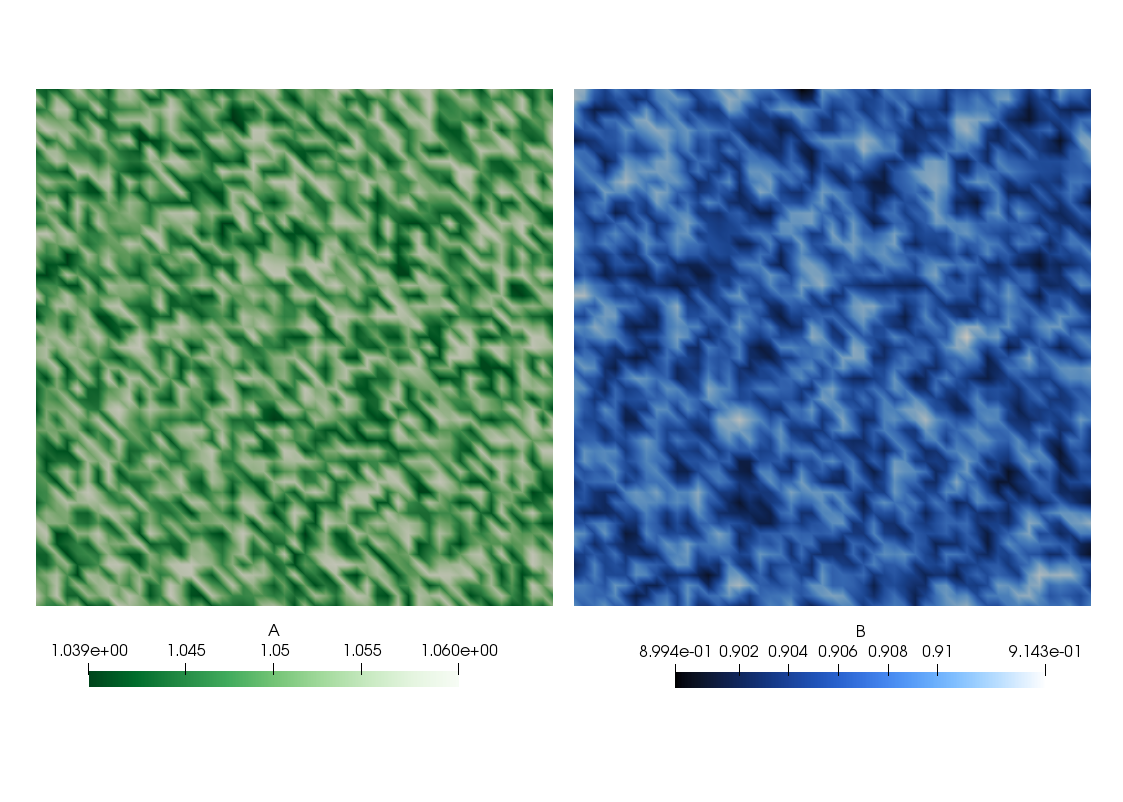
\includegraphics[width=6cm]{python_codes/fieldstone_130/results/AB_000}
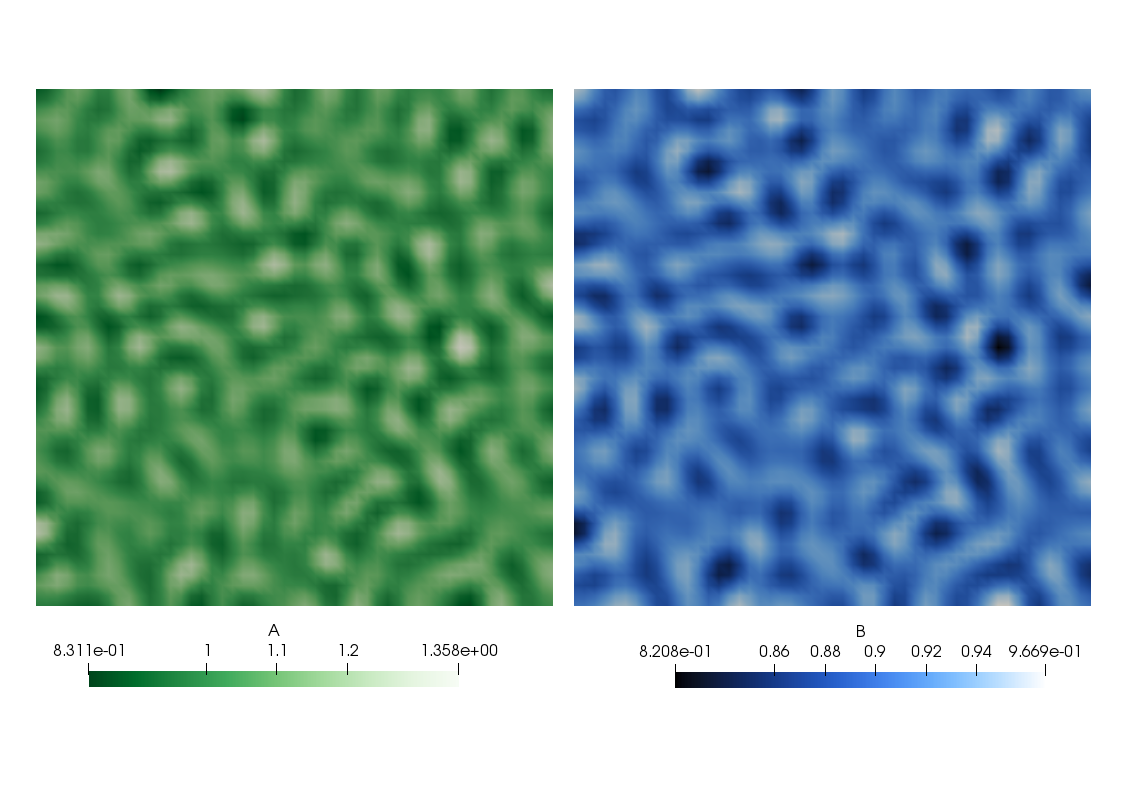
\includegraphics[width=6cm]{python_codes/fieldstone_130/results/AB_200}
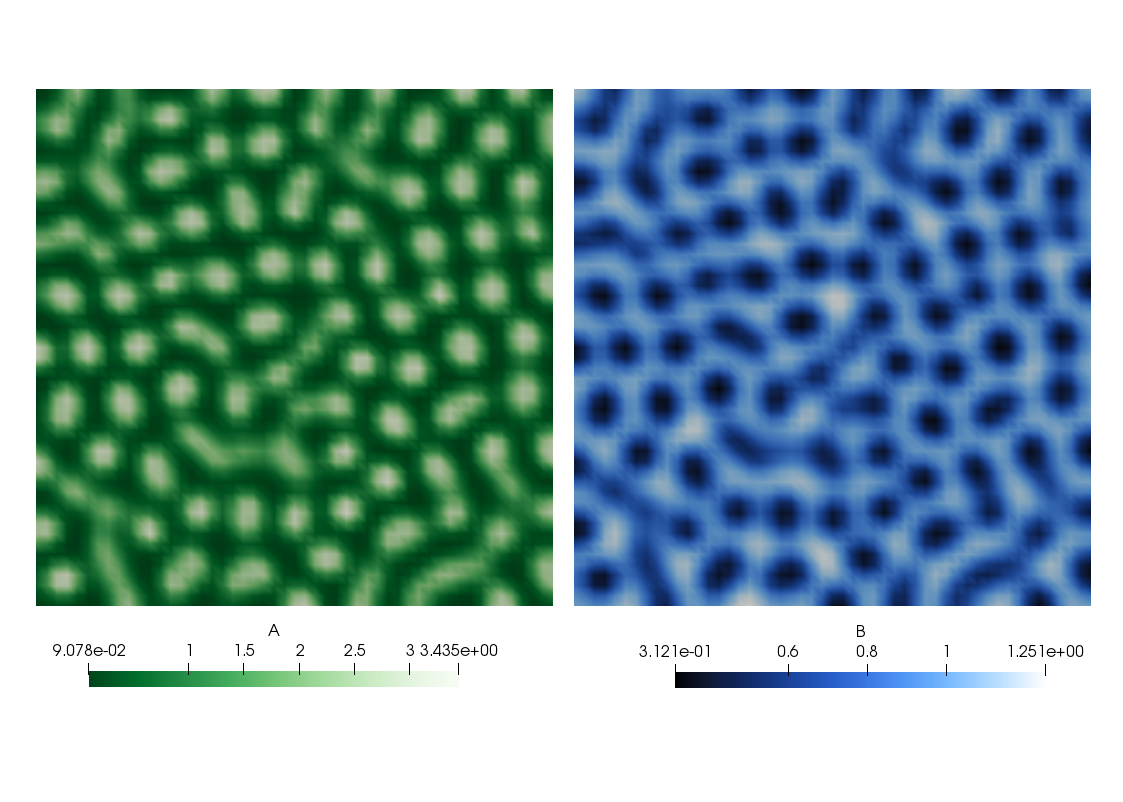
\includegraphics[width=6cm]{python_codes/fieldstone_130/results/AB_400}
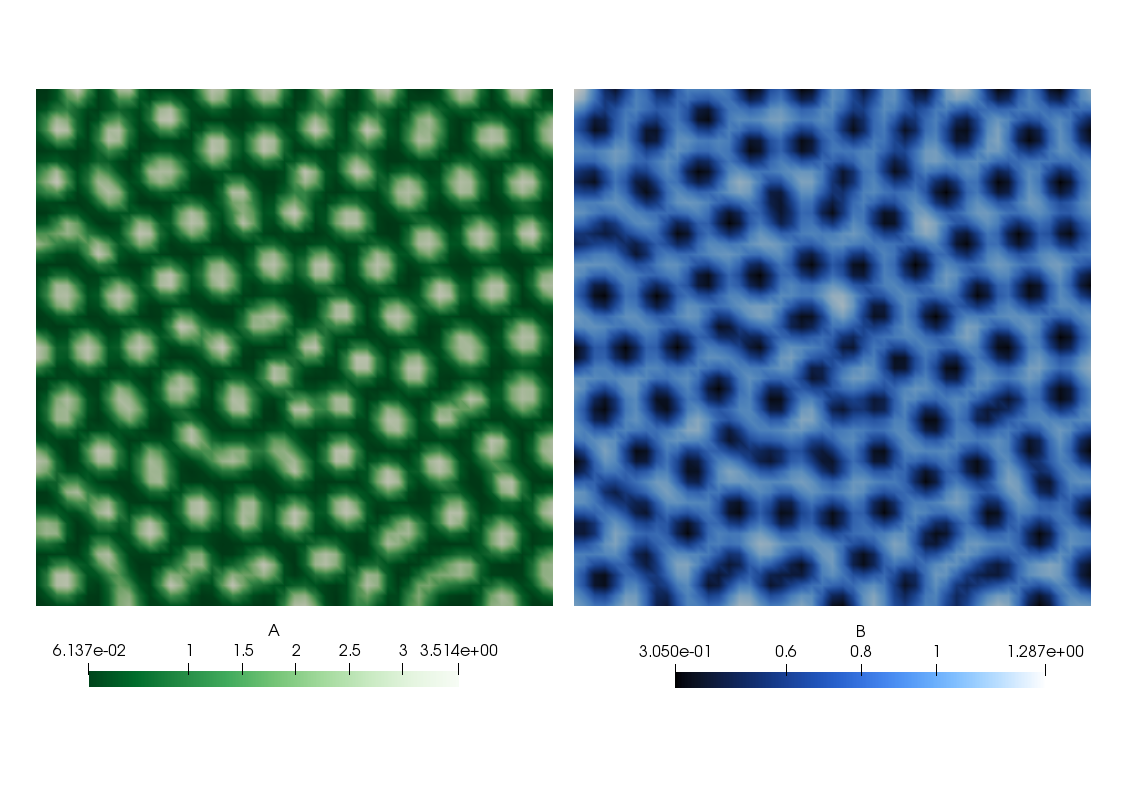
\includegraphics[width=6cm]{python_codes/fieldstone_130/results/AB_600}
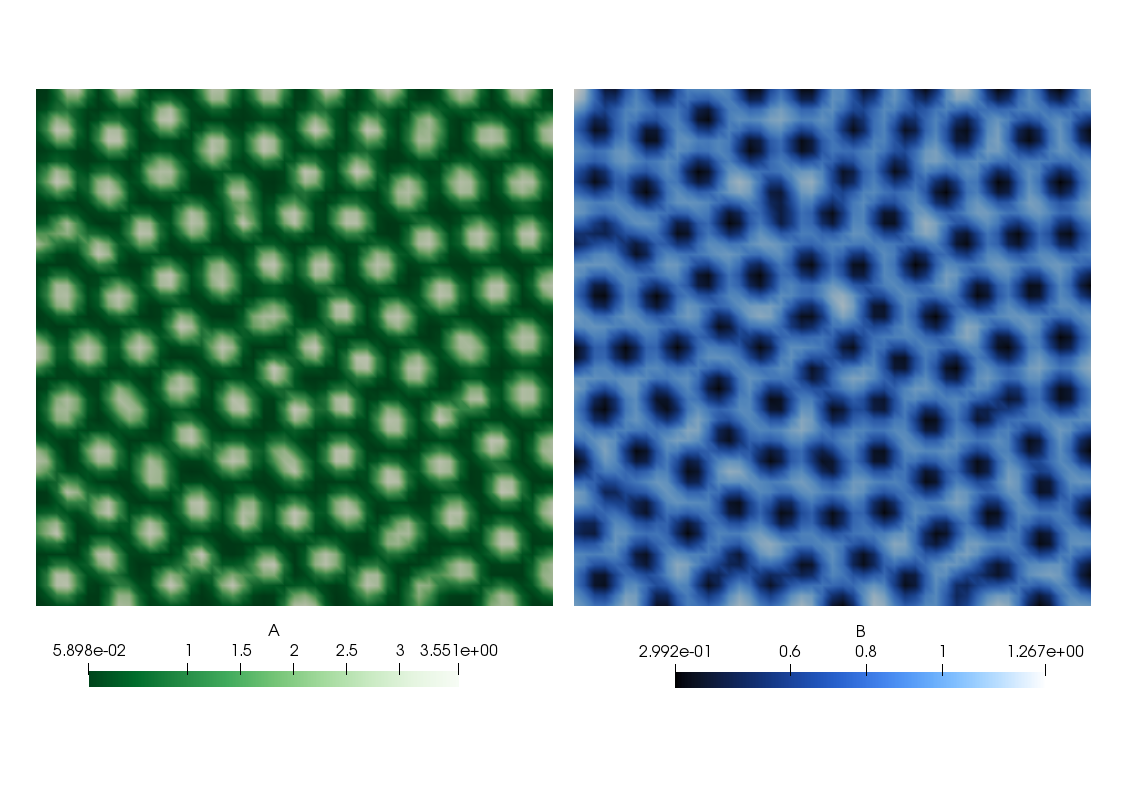
\includegraphics[width=6cm]{python_codes/fieldstone_130/results/AB_800}\\
{\captionfont phases $A$ and $B$ at time steps 0,200,400,600,800.}
\end{center}


\begin{center}
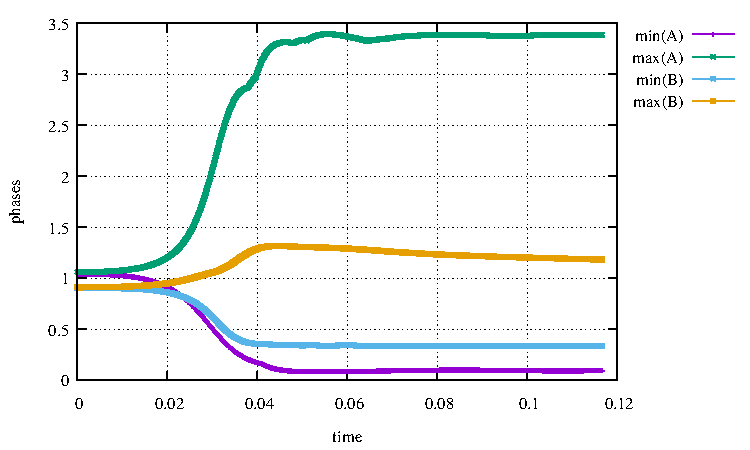
\includegraphics[width=10cm]{python_codes/fieldstone_130/results/stats_AB}
\end{center}
